%----------------------------------------------------------------------------------------
%   Theoretical Framework (Probleemanalyse)
%
%----------------------------------------------------------------------------------------
\chapter{Theoretical Framework}

%----------------------------------------------------------------------------------------
%   Introduction
%----------------------------------------------------------------------------------------
\section{Introduction}
To determine the difference in workload an in-depth review of Peppr's current workflow is needed. In this section, a deep-dive into the currently used process is exhibited, split into three sections. Firstly, a detailed outline of the 3d process will be described in the graphics section. Secondly, a peek into the software development process will be described in the software section. The split into these components will make it easier to determine possible sections of improvement later on. Third and final, a brief overview of the technology proposed by Peppr.

%----------------------------------------------------------------------------------------
%   Workflow
%----------------------------------------------------------------------------------------
\section{Workflows}
Peppr has done these projects and finds that the usual way of building consist of two main parts. The images and the software. The current process is outlined below. 

An example shall be used in the context of this thesis. Please note that this process is the way Peppr handles projects like this, and, while they did try to optimise it, this does not mean it is the perfect way to tackle such a project. The focus of the thesis is not on optimising the current workflow. The example project follows below.

\say{
A chair manufacturer wants a product configurator for one of their most popular chairs. It has 25 different colour options and has 3 different subframes. Two of the subframes are steel and can be either black or plain. The last frame is made out of wood.
}


%----------------------------------------------------------------------------------------
%   Graphics
%----------------------------------------------------------------------------------------
\subsection{Graphics}

%----------------------------------------------------------------------------------------
%   Image Planning
%----------------------------------------------------------------------------------------
\subsubsection{Image Planning}
Product configurators may have to deal with an exponentially growing set of options. Peppr always checks if these image sets can be split into separate components. This makes the set smaller and easier to maintain. Below is a summary of the option set, split out per configurable option so we can start calculating how many images will be necessary.
\begin{itemize}
	\item 25 colours - (\( \alpha \))
	\item 3 frames - (\( \beta \))
	\item 2 frame colours - (\( \gamma \))
\end{itemize}

To calculate the full amount of options ($y$), we can use the following formula:
 
\[ y_1 = \alpha \cdot \beta \cdot \gamma\]
\[ y_1 = 25 \cdot 3 \cdot 2\]
\[ y_1 = 150\]

Adding just one extra colour option to the seat more adds 6 extra renders ($1 \cdot 3 \cdot 2$). While this does not seem like much, these renders are built from several different files. This means that, depending on the way the files that create the images are split up, an artist has to open either 6 or 25 different files and do the edit 6 or 25 times. Here, 6 seems easier, but might prove difficult later on when trying to change something else.
In some cases one might be able to get around it using layered images. In this case, splitting up the chair into a layer that contains the seat and one that contains the frame will get us the following formula:

\[ y_2 = \alpha + (\beta \cdot \gamma)\]
\[ y_2 = 25 + (3 \cdot 2) \]
\[ y_2 = 31\]

This decreases the amount of renders drastically. Unfortunately, in some cases this is not possible. Sometimes, one of the pieces of the model (frame for instance) is both in front and behind other objects. This makes it difficult to create an image set for those pieces. For instance, when there is a second seat that is transparent at certain points, then it needs to show the frame through the seat, this means a second image set is needed for the frames. The biggest issue in this case however (and why it will not work for this configurator) is that the seating area of the chair will be reflected in the frame. So when the colour of the seat changes, the reflections should be updated as well. As such, while adding the frame to a separate layer is a possibility, it would still need a version for every seat colour. Also, creating new layers does add complexity and constraints in the software.
\newline
Apart from difficulties in the 3d process, these layers need to be added to the software as well. Either by creating an API that serves the layers as one image (\cite{bugaboo} ), or by stacking the images client-side. The user will notice this option though, as it slows things down. This is fixed with the adoption of HTTP 2.0. This pipelines the http-requests, reducing latency (\cite{latency}).

%----------------------------------------------------------------------------------------
%   Modeling
%----------------------------------------------------------------------------------------
\clearpage
\subsubsection{Modeling}

Step two in the process is modeling, where an artist makes a virtual model. Polygonal modeling is the most common form of 3d modeling used at Peppr. This means the model will eventually be represented by an array of 3 dimensional points (or vertices). The vertices are connected by lines and those lines make up the surface of the model. There are multiple ways of creating these models. One way is for an artist to 'draw' those polygons from scratch. Another option would use 3d scanning services or even simulations to build the 3d models.
As seen in Figure \ref{figure:modeling}, every single square in that model is one of these polygons, which in this case, are drawn from scratch.

\begin{figure}
\centering
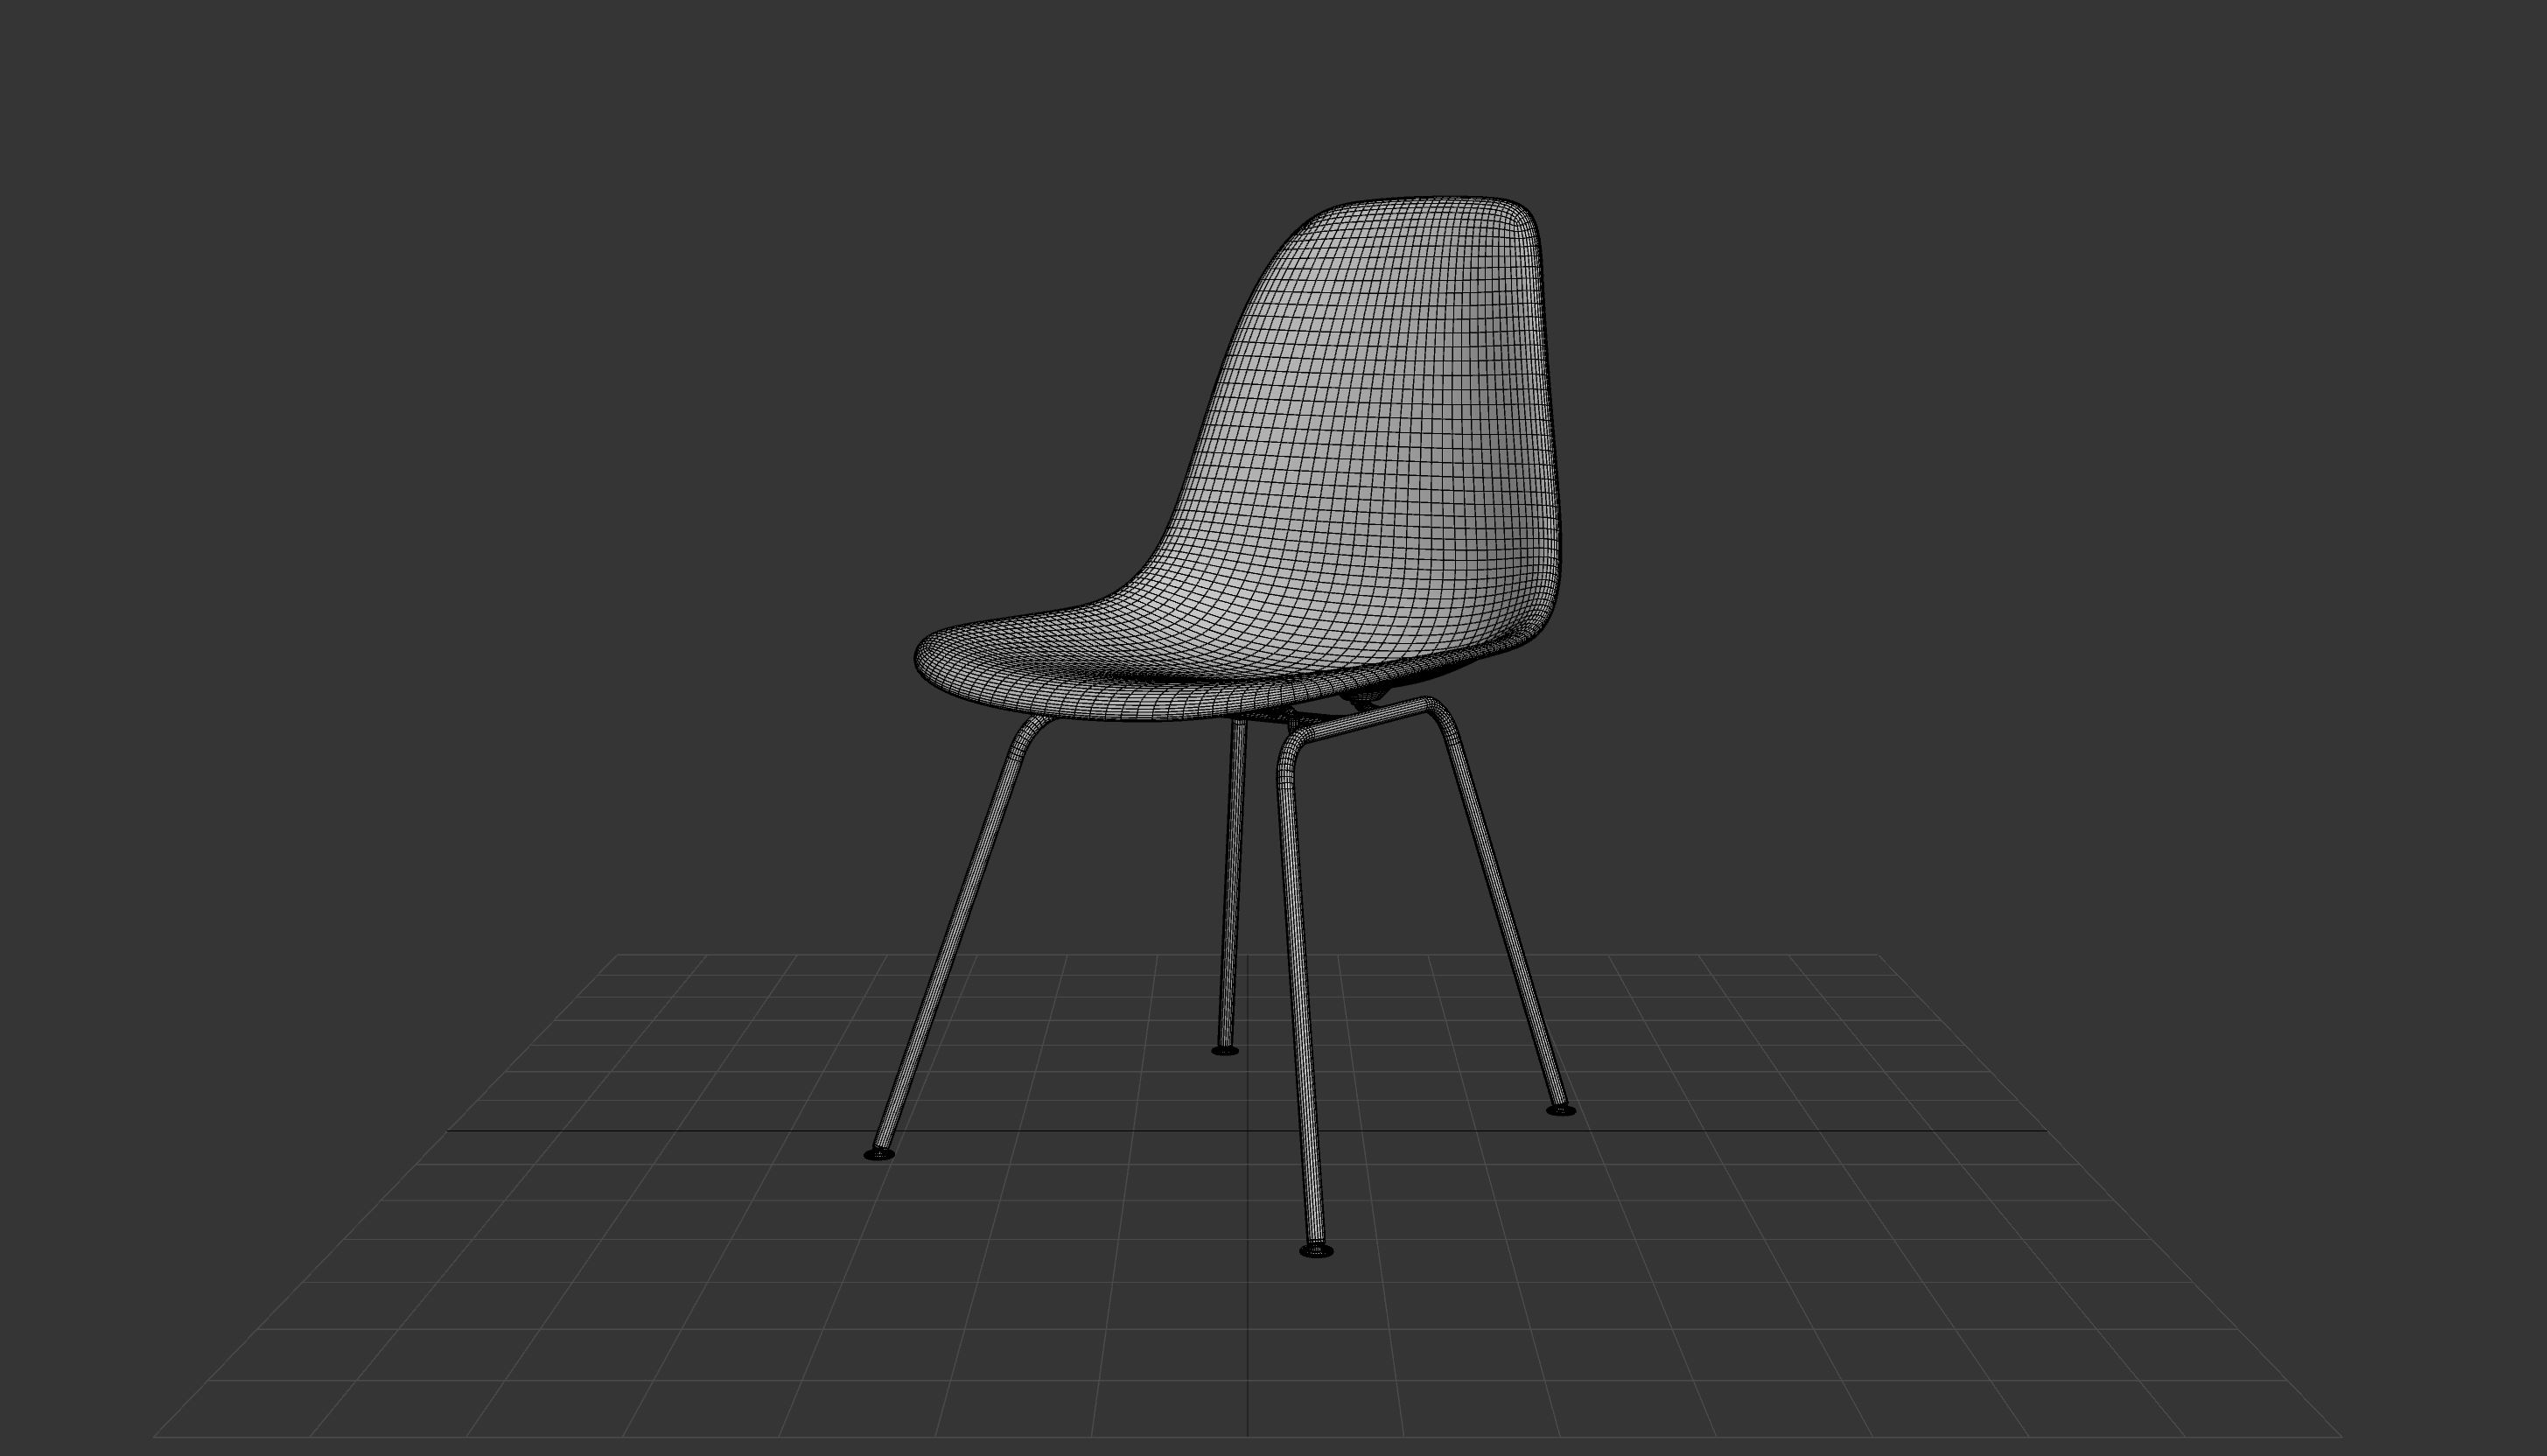
\includegraphics[width=16cm]{images/modeling}
\caption{Modeled Chair}
\label{figure:modeling}
\end{figure}

%----------------------------------------------------------------------------------------
%   Lighting / Shading
%----------------------------------------------------------------------------------------
\clearpage
\begin{figure}
\centering
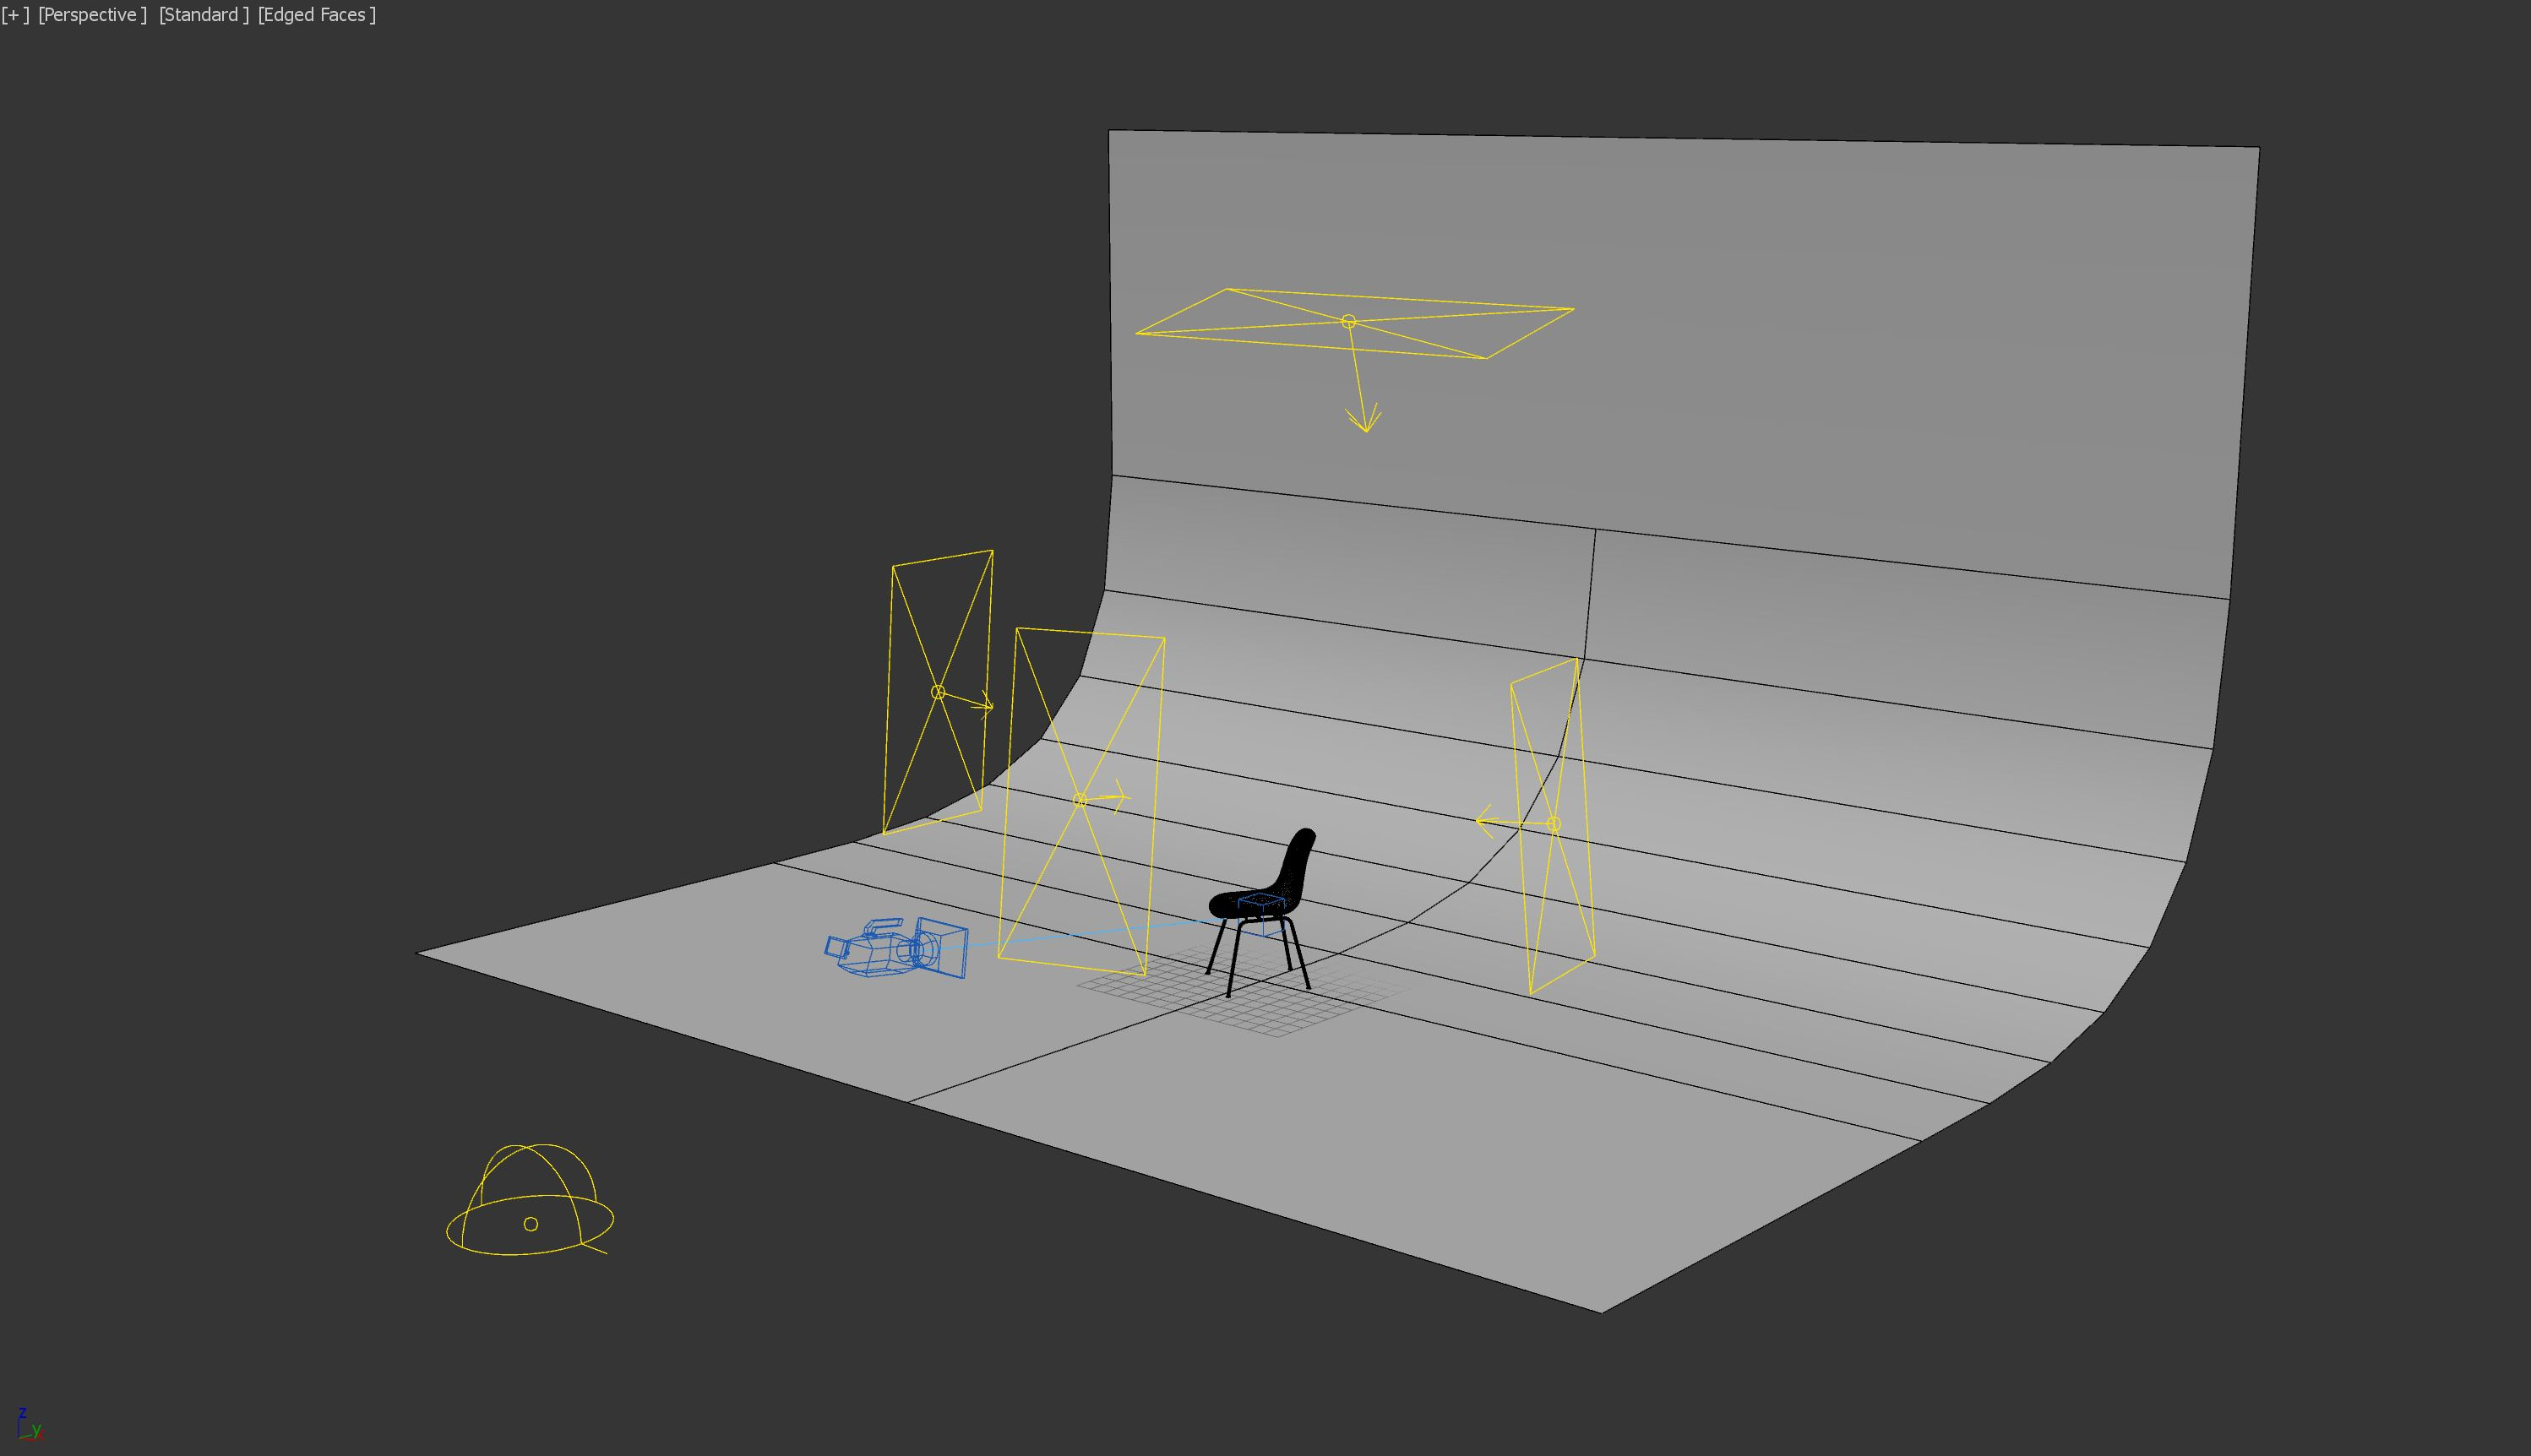
\includegraphics[width=16cm]{images/lighting}
\caption{Lighting Setup}
\label{figure:lighting}
\end{figure}


\subsubsection{Lighting}

\begin{wrapfigure}[12]{r}{10cm}
\vspace{-1cm}
\centering
\includegraphics[width=9cm]{images/lighting_rendered}
\caption{Rendered Lighting Setup}
\label{figure:lighting_rendered}
\end{wrapfigure}

Once the model has arrived in the lighting department, the model is placed in a virtual photography studio to add lighting. As seen in Figure \ref{figure:lighting}, there are 5 lights in the current setup. One is a dome light that simulates the environment using a so-called 'High Dynamic Range' (HDR) range image. Normal jpg images (ones that are used for the web for instance) are 24 bit. As an image is separated into a red, green and blue channel, every colour has 8 bits of information available. This means a jpg image is able to show 256 ($2^8$) shades per colour, so a normal JPG image, having three colour channels (8 bits per channel), has $16.777.216$ possible colours in total ($256^3$). \newline
The HDR images are mostly encoded in a 32 bits per pixel option. In laymen terms, this means that an HDR image has more colours per pixel ($2^{32}$ per colour channel, so $4.294.967.296$), than a JPG image has in total. The total would amount to a staggering $4.294.967.296 ^ 3$. In practice, this means that the extremely bright parts of the image can be used to extract lighting information. The HDR image is mapped onto a spherical dome that in term will simulate an actual environment without the need to add extra lights. In this case, Peppr used an HDR of an actual studio environment.
 The other four images are used to light the model to perfection. One light at the back for the background, one in front to have highlights and two diffuse boxes on the side to get the model to stand out from the background.

%----------------------------------------------------------------------------------------
%   Lighting / Shading
%----------------------------------------------------------------------------------------

\subsubsection{Shading}

\begin{wrapfigure}[20]{r}{10cm}
\vspace{-1cm}
\centering
\includegraphics[width=9cm]{images/rendering}
\caption{Rendered image with shaders}
\label{figure:lighting_rendered}
\end{wrapfigure}

Once properly lit, an artist will start shading the model. In this process, life-like materials are added to the object to make it come alive. This process can be tricky as there are lots of variables involved. Setting the colour is relatively straight-forward, but when it comes to reflections or refractions, the options become more elaborate because every material reflects in a different way. Not only the amount of reflectivity needs to be adjusted, but also the amount the reflections are blurred (on rougher surfaces for instance). Next to that, materials (usually) reflect differently when observed from different angles. These values are directed by the materials Index Of Refraction (IOR \cite{refractiveIndex}, more on that in the render section (\ref{sec:render})). The Index Of Refraction is combined with Fresnel equations (\cite{fresnelEquations}) for a proper reflectivity per angle. The same thing counts for Refractions.
Another important consideration when defining materials is the objects texture. There are few materials that are completely smooth. The plastic in Figure \ref{figure:lighting_rendered} has a minute texture. This adds a tiny bit of extra realism.


%----------------------------------------------------------------------------------------
%   Rendering
%----------------------------------------------------------------------------------------
\subsubsection{Render}
\label{sec:render}
This is where things get together and at this point the calculations are made that create an actual image from the 3d model. There are two sides to this, the technical settings of the render-engine used and the structure of the file / timeline.
\newline
\textit{Render-engine}
\newline
Peppr opts to use third party render-engines for their projects, mostly for speed and quality optimizations. While having more options, they are also more difficult to use. With most of Peppr's projects, there is an equilibrium between quality and render-times. The render-times have to do with the difficult nature of light, reflections, refractions and the anti-aliasing of the image. Light, for instance, obeys the 'inverse square law' (\cite{inverseLightLaw}), which means the intensity of light decays the further it gets from the point-of-origin. Using one light, this is quite easy, but imagine having 3 or 10 lights interacting at different intensities from different locations. On top of that, light bounces around. The render-engine calculates the point of impact, checks the properties of the materials it hits and radiates the light back from the surface. The directionality of these light reflections is where lots of rendertime is spent. The more straightforward the reflections, the easier. A mirror will reflect the light at the same angle of incidence, but when the material is rough, the rays get scattered. For this, the render-engine will 'shoot' out multiple rays (for example 50), up to a predefined number of times. In practice, this means that when one ray bounces on a rough surface, it spawns 50 new rays. If all of those rays bounce off of a rough surface again, the number of rays will amount to $50 \cdot 50$. With every bounce, this will increase exponentially.

Refractions are even more difficult because of the Index of Refraction. This index specifies change of angle in a lightray when it goes from one material to another (\cite{refractiveIndex}). Water (at 20\degree C) for instance, has an IOR of 1.333 (\cite{waterIOR}). This means that, next to the light rays bouncing, they can also change direction.

The third and last part that makes rendering images a lengthy task is anti-aliasing. Anti-aliasing is a way of making the images 'smooth'. It has to do with the square nature of pixels. A diagonal line will not look smooth if it is just one line of pixels. Instead, the pixels directly surrounding it get a semi-translucent fill, which makes the line look smooth. The blending of colours (while not overdoing it) is the anti-aliasing part, this is a very slow process that demands high computing powers.

Peppr uses these intricate render-engines to fine-tune the render-settings. For studio setups, where direct lights are the most important light sources, Peppr might choose to use a set of settings where the secondary bounces of light are of lesser quality than, for instance, a 3d interior scene, where most light comes from the light bouncing on the floor (indirect).
\newline
\newline
\textit{Automation}
\newline
Sometimes it is easier to render the whole sequence with every configuration. Other times, it is easier to render just one point-of-view at a time. In the case of the shirt configurator, every shirt had many different collars, sleeves, buttons, but also colours. There are numerous ways of splitting this up, automating the process as much as possible. Most 3d modeling applications have a way to animated models, either frame-by-frame or using blending. By changing one aspect of the model for every frame and rendering it out as an image sequence, the rendering process can be partly automated. The result of this is a sequence of images where one aspect of the model is changed with every image. The problem with this is that it will always be a choice of lesser evils. While rendering the sequence, it is key to look at the biggest common denominator and use that as a base. In the shirt configurator case, this meant splitting it up so that there is a file for every colour. This means the file structure is somewhat logical (a file for every colour) and changing one aspect is relatively easy. Unfortunately, this is by no means ideal. Some changes have to be done 25 times (once for every colour).


%----------------------------------------------------------------------------------------
%   Post Production
%----------------------------------------------------------------------------------------
\subsubsection{Post Production}
\begin{figure}
\centering
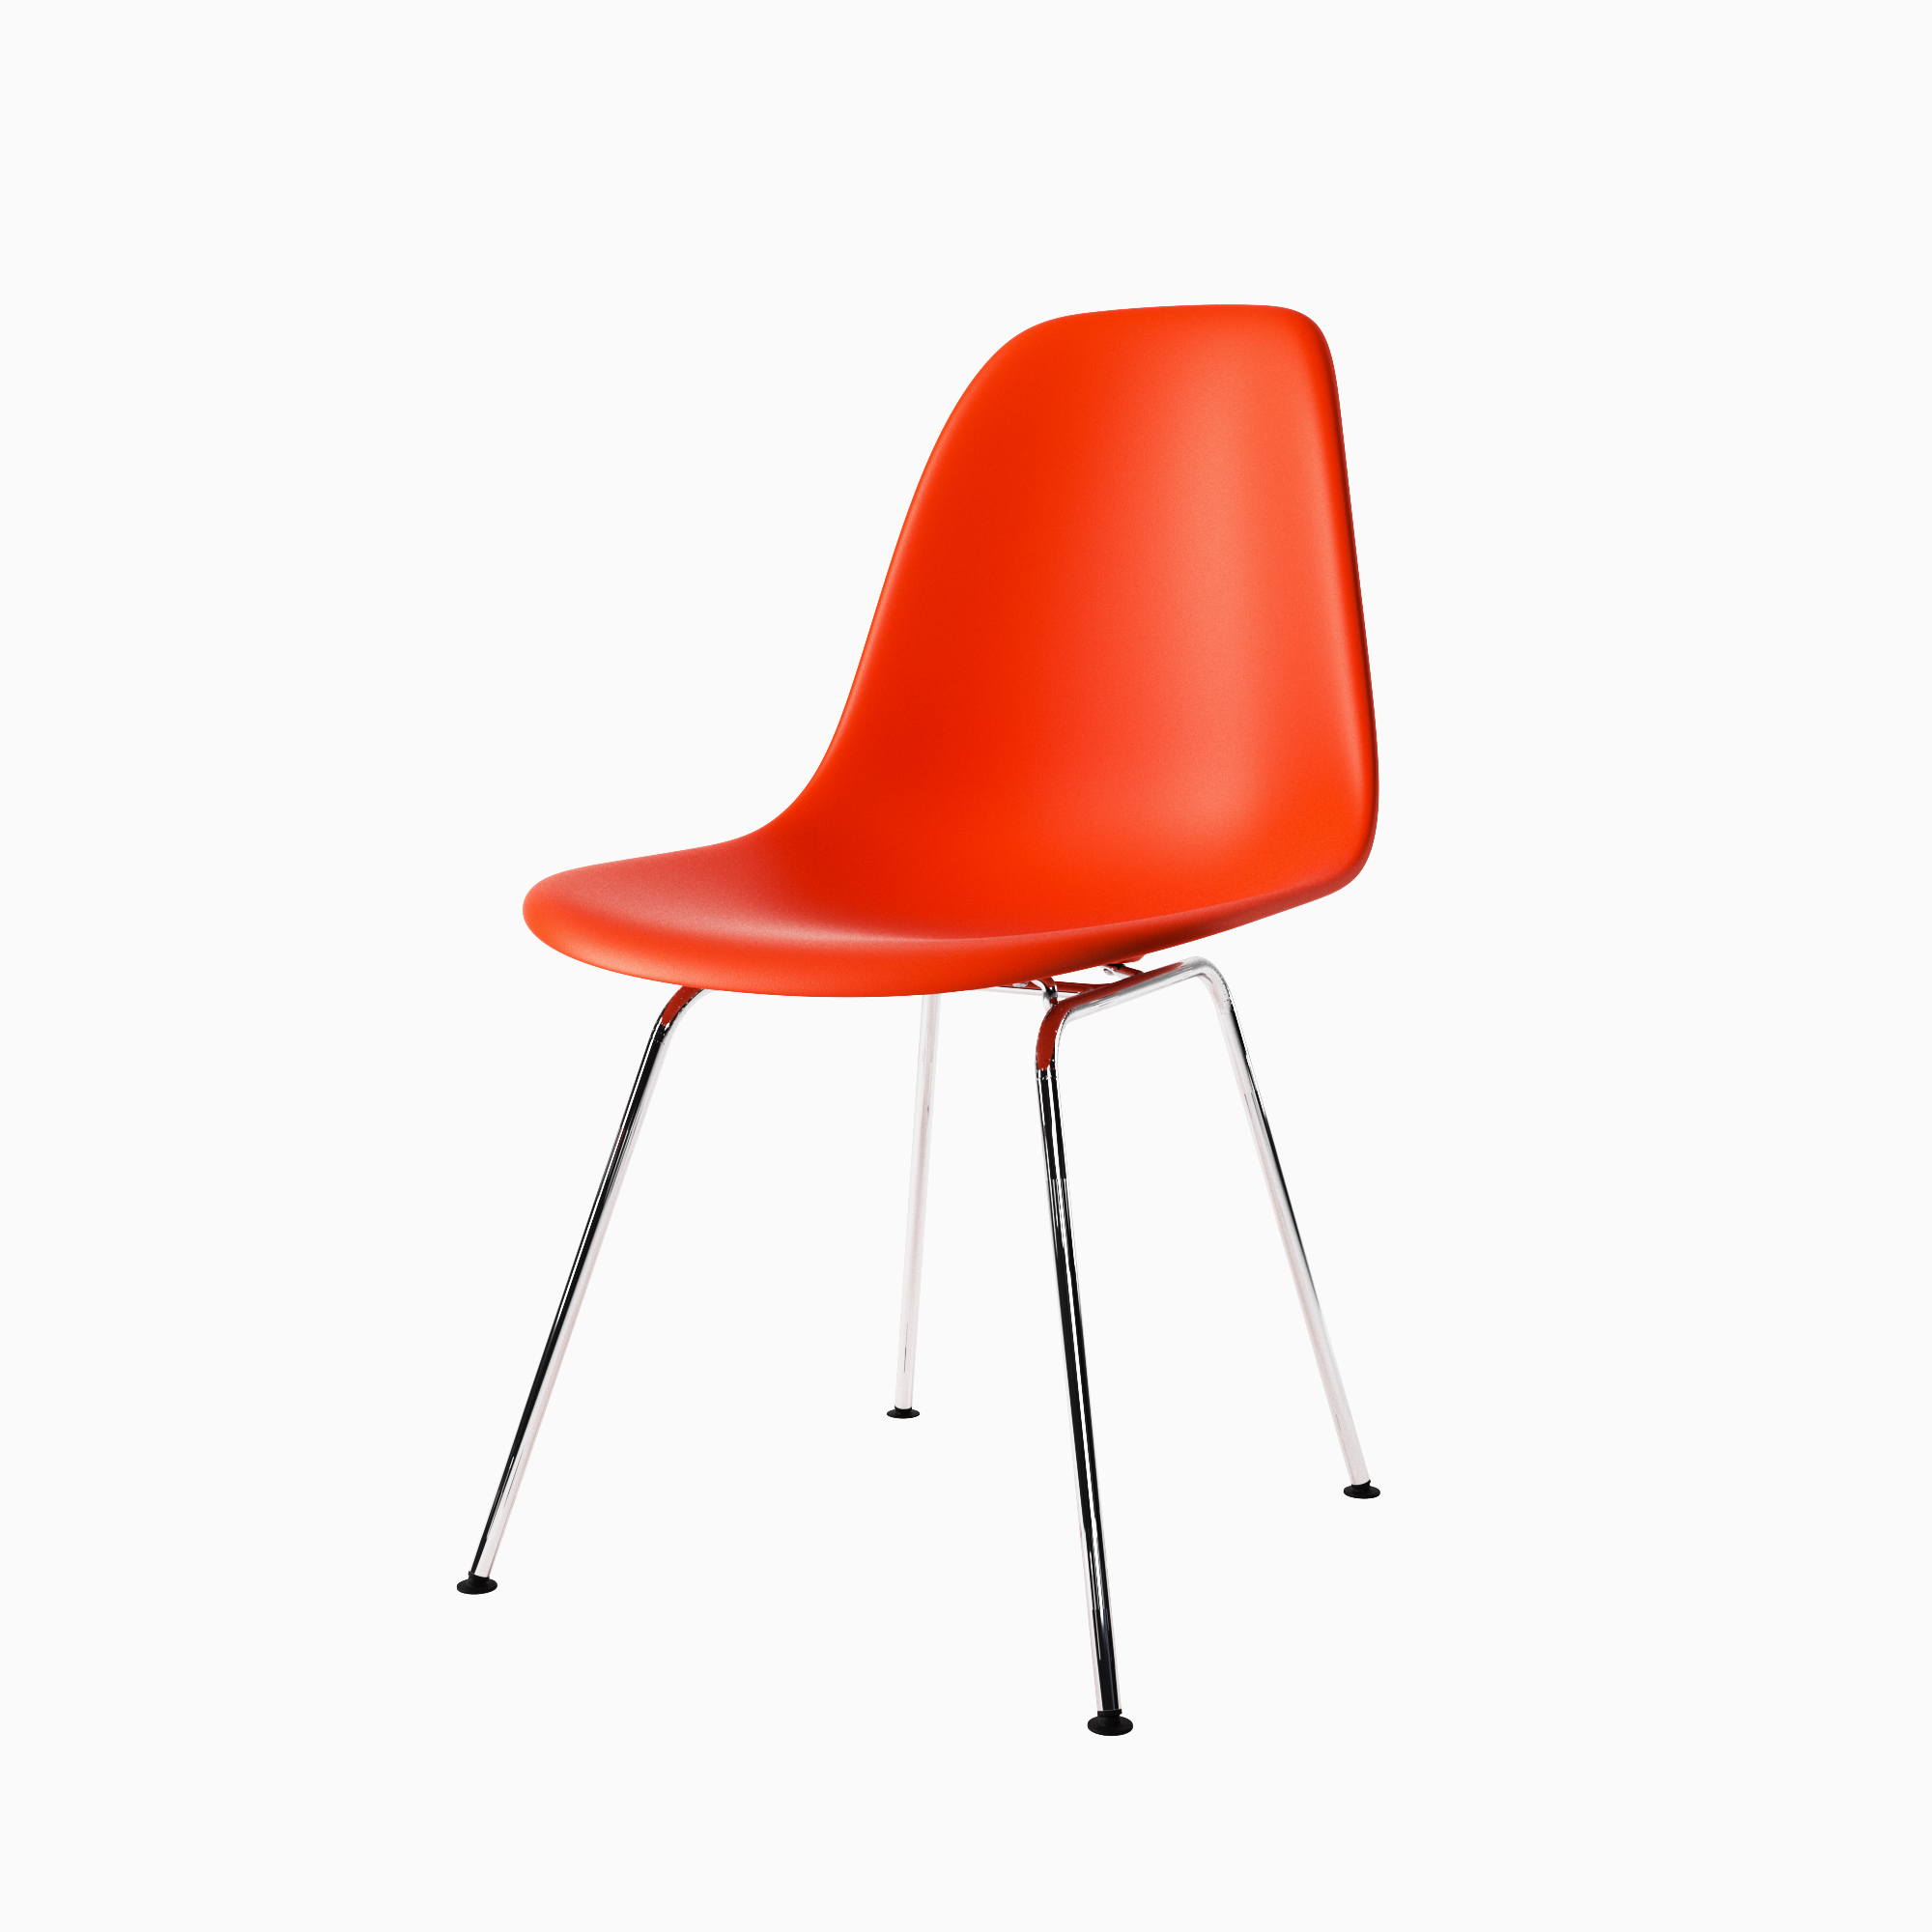
\includegraphics[width=16cm]{images/post}
\caption{The final rendered image after post-production}
\label{figure:post_production}
\end{figure}

Every 3d model needs a bit of post production. There are two main reasons for this, one is to make the image look better (with applied color correction), the other when the model is rendered using layers and those need to be split into several image files. The layers are rendered as a black and white maps where the white part of the image is the part that is visible in that specific layer. This is the step where the images would be split into those layers. In case of the shirt configurator this has partly been automated. Using the same animation principles highlighted in the Section \ref{sec:render}, Peppr made sure the post-production files would have all the options for for a single colour shirt so they could easily copy changes from one set of colours to another. In Figure \ref{figure:post_production}, the background has been removed and some minor colour corrections have been made to make the colour stand out a bit more.
\newline
%----------------------------------------------------------------------------------------
%   Compression
%----------------------------------------------------------------------------------------
\subsubsection{Compression}
When using the final images on the web (which was the case in this instance), small file sizes are important. Having the user download 50mb worth of images when opening a site is not a good idea, this will be slow and will not be nice for users that have a datacap on their subscription. According to the W3C guidelines, the file size should not exceed 20 kilobytes (\cite{pageFileSizeLimit}). This is were compression comes in. Every image is compressed for a fast download, while remaining good quality. The 20 kilobytes stated by the W3C guidelines are unfortunately not an option as one image is probably bigger than that, but a best effort to make the images as tiny as possible is still required.
A couple of things can be done to achieve this. First and foremost the image should be the proper size. The rendered image is 2000 x 2000 pixels (w x h). The images for the shirt configurator by Peppr were only required to be 800 x 500. Making the image 800 x 800 reduced it from 445kb to 91kb. This is a big change, but  proper compression can take this even further. Using an application like ImageOptim (\cite{imageOptim}), the size is further reduced to a mere 68kb. The savings from 91kb down to 68kb do not sound like much, but when there is an image set of hundreds of images, shaving 25\% off of the filesize counts.

%----------------------------------------------------------------------------------------
%   Software
%----------------------------------------------------------------------------------------
\subsection{Software}
Now that the graphics process has been described, it is time to dive into the software development cycle. The steps Peppr currently uses in their pipeline are outlined below.
​
%----------------------------------------------------------------------------------------
%   Functional Requirements
%----------------------------------------------------------------------------------------
\subsubsection{Functional Requirements}
Functional requirements help map out required functionality of an application. In an agile (\cite{agileUserStories}) working environment, these are 'user stories'. Peppr prefers the term requirements. They generally use the same notation. \newline

\say{\textit{As a <type of user>, I want <some goal>, so that <some reason>}}\newline

In the context of the configurator specified above, a requirement could be: \newline

\say{\textit{As a \textbf{User}, I want \textbf{to be able to save my configuration}, so that \textbf{I can later continue were I left off with my configuration}}}\newline

%----------------------------------------------------------------------------------------
%   Technical Requirements
%----------------------------------------------------------------------------------------
\subsubsection{Technical Requirements}
Contrary to popular belief, these requirements are not the implementation details of the functional requirements. They are the requirements of the system itself. The technical requirements handle things like performance, availability and security. In the official agile requirements, they are put in to a summarized list \cite{agileTechnicalRequirements}, but Peppr opts to use the same format as the user stories. \newline


\say{\textit{A \textbf{<type of system>} should \textbf{<do something>} so that \textbf{<some reason>}.}}\newline

Peppr uses this to differentiate between different types of systems. An example of a technical requirement can be found below. This specific one has to do with limiting an API's response time (\cite{responseTimes}).

\say{\textit{An \textbf{API} should \textbf{respond within 300ms} so that \textbf{the user feels in control of the application at all times}.}}\newline

%----------------------------------------------------------------------------------------
%   CMS
%----------------------------------------------------------------------------------------
\subsubsection{Content Management Systems}
A content management system (CMS) has basic functionality built in (like user management or file handling). It does however, requires the developer to work in the way the system intended, which may prove inflexible. Another option is to go with a system that is written from the ground up. It will be much leaner and quicker when deployed, but will not be as mature as a popular CMS. So if the system is not built right, it may result in a buggy experience for the end user. In Peppr's case, a CMS called Magento was used during implementation. One thing to keep in mind: In case of a custom application, a back-end needs to be developed as well.
%----------------------------------------------------------------------------------------
%   UX Development
%----------------------------------------------------------------------------------------
\subsubsection{User Experience Development}
While the term 'User Experience' (UX) gets thrown around a lot, the UX (User Experience) covers not only the User Interface of the application. It is a broader term to describe how users undergo the experience of using, in this case, the product configurator. It is how they learn to use the product configurator. Next to that, is should cover how the application can help the user in the best possible way to do so. For one, so the user can complete a configuration, but also that he / she does so with joy. Don Normal (\cite{userExperience}) says: \newline
\say{\textit{The first requirement for an exemplary user experience is to meet the exact needs of the customer, without fuss or bother. Next comes simplicity and elegance that produce products that are a joy to own, a joy to use. True user experience goes far beyond giving customers what they say they want, or providing checklist features.}} \newline
In other words, the user experience is not only about helping the user to meet his or her goal. It is to go beyond that, and make the experience joyful.

%----------------------------------------------------------------------------------------
%   Back-End Development
%----------------------------------------------------------------------------------------
\subsubsection{Back-End Development}
Techopedia (\cite{backendDevDefinition}) states that a back-end developer's task is to develop and maintain a logical or computational back-end for a website. Focussing on C++, C\#, Java or another high-level programming language. Another Definition (\cite{backendDevDefinition}) states back-ends are mostly developed using either Ruby or Python.
In reality, any programming language that can interact with a database can act as a back-end. For instance, the 'Dollar Shave Club' uses 6 languages in their infrastructure (\cite{dollarShaveClubBackEnd}). 'Uber', uses a completely different stack (\cite{uberBackEnd}).
Peppr generally uses a microservices architecture for their apps (\cite{microservices}). This pattern allows the use of different applications. So, Peppr can build each application using a specific language and with a specific target in mind. Imagine a configurator needs to stack images but also needs a realtime chatbot. Peppr will be able to handle the high concurrency using something like Elixr (\cite{elixr}). The realtime chatbot will then be made with Firebase, a realtime socket service (\cite{firebase}).

%----------------------------------------------------------------------------------------
%   Front-End Development
%----------------------------------------------------------------------------------------
\subsubsection{Front-End Development}
According to Wikipedia, a Front-End Developer (\cite{frontEndDevDefinition}) produces the client-side interface. Wikipedia states that they use HTML, CSS and Javascript. However, anno 2016, Front-End Development has become quite a bit more than just that (\cite{javascriptAnno2016}). For relatively complex projects like configurators, building a front-end can be a daunting task. In a single page web application, one wants to serve the changes to the user instantly, without a page refresh. This requires a so-called asynchronous approach. 
Building an asynchronous application can be done in many ways. The most convenient way is to build a Single-Page-Application (SPA). This gives the user a desktop-like experience (\cite{singlePageApplications}). As stated on Wikipedia, there are some caveats to this, like search engine optimisation, speed and browser history. Fortunately, there are frameworks to help build an SPA. Anno 2017, the field of Front-End Development is clouded with frameworks to help build these types of applications. MeteorJS, React, Angular, Vue and many more (\cite{frontEndJavascriptFrameworks} ).
Peppr develops most of their applications using Angular. They found that code maintenance and separation of concerns are best realised using a Model-View-Controller (MVC) type setup (more on that later). And they decided to use the AngularJS framework to create that setup.


%----------------------------------------------------------------------------------------
%   OpenGL & WegGL
%----------------------------------------------------------------------------------------
\clearpage
\section{OpenGL \& WebGL}
Peppr suggested the technology that possibly holds the answer to a better configurator is OpenGL and its web counterpart; WebGL.
The first version of OpenGL was released March 2011 (\cite{openGLsite}). It is a software interface to allow programmers to interact with graphics hardware (\cite{openGLSpecification}). It is essentially an API acting as a middle man between software and hardware. In practice, this means that programmers will need only little (to no) hardware knowledge while still being able to tap into the hardware calculation capacity. Normally, starting up an OpenGL application, it creates a window inside of the application that ties into the framebuffer (\cite{framebuffer}), basically a piece of RAM memory containing the bitmap. The application then holds a GL context (basically all the OpenGL state data for this frame buffer), and the OpenGL commands can be used to modify and interact with the contents.

To use OpenGL on the web, one needs an API that interacts with OpenGL. This can be done server-side, with the result of the graphics hardware framebuffer being sent to the user, which will not require any computing power on the user's side (\cite{CRRS}). This means that any language parseable on a server that can send data out and has an OpenGL enabled graphics card, can be used. Even though this article stems from 2008, the problems stated with latency still exist today, even when taking their suggested and tested optimisations into consideration. Next to that, servers that have graphics cards are relatively expensive. Another option is client-side rendering. With the increase in speed for customer technology and the rise of smartphone usage, the amount of devices that have a graphics card and can use this technology increases. Unfortunately, it is not possible for (most) webbrowsers to directly communicate with the OpenGL framebuffer. Fortunately, there is a solution: WebGL.

\say{WebGL is a cross-platform, royalty-free web standard for a low-level 3D graphics API based on OpenGL ES 2.0, exposed through the HTML5 Canvas element as Document Object Model interfaces.}
\cite{webGL}

WebGL technology renders from the graphics hardware (just like OpenGL). The key difference is that the API is exposed to an HTML5 canvas element. This means the framebuffer is not opened into an application window, but into an HTML5 canvas element. While this solves the issue of running GL content client-side, GLSL (the language used to interact with WebGL \& OpenGL) does not make it into the Stack Overflows Annual Survey (\cite{stackoverflowDeveloperSurvey}). This does imply it would be hard (and expensive) to find competent developers that can built an application using this technology.
Fortunately, Peppr found a library that makes this easier. It uses the most popular language in the survey (Javascript). "Three.js", as the library is called, filled the last gap in client-side OpenGL / WebGL content. It supplies the option to code WebGL content with javascript, so there is no need for GLSL. The question remains, while javascript itself is adopted in most modern browsers (\cite{javascriptSupport}), will the three.js library work bug free in those browsers?


\newpage





